\documentclass[sigconf]{acmart}
\usepackage{graphics}
\usepackage[utf8]{inputenc}
\usepackage{algorithm}
\usepackage{algorithmic}
\usepackage{url}
\usepackage{setspace}

\linespread{1.5}

\makeatletter
\def\subsubsection{\@startsection{subsubsection}{3}%
  \z@{.5\linespacing\@plus.7\linespacing}{.1\linespacing}%
  {\normalfont\itshape}}
\makeatother

\begin{document}
\title{Parallel Algorithm for Stable Marriage}

\author{Zeid Ayssa}
\affiliation{
    \institution{University of Texas at Austin \\ Dept. of Electrical and Computer Engineering}
}
\email{azeid@utexas.edu}

\author{Tyler King}
\affiliation{
    \institution{University of Texas at Austin \\ Dept. of Electrical and Computer Engineering}
}
\email{tylerhk93@gmail.com}

\author{Guillermo Le\'on}
\affiliation{
    \institution{University of Texas at Austin \\ Dept. of Electrical and Computer Engineering}
}
\email{gleon@utexas.edu}

\author{Jesus Valenzuela}
\affiliation{
    \institution{University of Texas at Austin \\ Dept. of Electrical and Computer Engineering}
}
\email{javier.valenzuela@utexas.edu}

\begin{abstract}
The Gale-Shapley\cite{gale1962college} “propose/reject” algorithm is a well-known procedure for solving the classical stable marriage problem. In this paper a few alternatives for a parallel algorithm to solve the stable marriage problem are given. The worst case performance of our implementation is stated.    
\end{abstract}

\maketitle


\section{Introduction}
Algorithm alternatives considered during this research:\\

The stable marriage problem is defined as: Given N men and N women where each man ranks each women from 1 to N and each women ranks men from 1 to N, where 1 is the highest preference and N being the lowest preference. Marriages are one-to-one where one man can only be married to one women and vice versa. Additionally, a marriage is considered unstable if there exist match $\{M_1, W_1\}$ where $M_1$ prefers a another $W_2$ over his current match $W_1$ and $W_2$ prefers $M_1$ over her current match $M_2$. 





\subsection{Parallelization of Gale-Shapley}

The version of Gale-Shapley algorithm chosen to parallelize was the one given by Gusfield et al.\cite{Gusfield:1989:SMP:68392} in 1989. The algorithm is briefly described in Figure \ref{fig:my_label}.

\begin{figure}[h]
    
    \begin{algorithmic}
    \STATE $l \gets $all free men
    \WHILE{some man $m$ in $l$}
        \STATE $w \gets$ woman on $m$'s list to whom $m$ has not yet proposed
        \IF{$w$ is free}
            \STATE assign $m$ and $w$ (they are now engaged)
        \ELSE
            \IF{$w$ prefers $m$ to her fianc\'e $m\prime$} 
                \STATE assign $m$ and $w$, $m\prime$ is now free
            \ELSE
                \STATE $w$ rejects $m$, so $m$ is still free
            \ENDIF
        \ENDIF
    \ENDWHILE
    \end{algorithmic}

    \caption{Gale-Shapley Algorithm as described by Gusfield et al.}
    \label{fig:my_label}
\end{figure}

In order to have a good base line for comparing other algorithms we decide to not change this basic structure of the algorithm. Instead we opted for using concurrent data structures and synchronization mechanisms provided by the language we implemented all of these algorithms, Java. In the implementation section we go in further detail about the chosen concurrent data structures and mechanisms.

In Gale-Shapley algorithm, and man optimal, each women makes at most (men-1) rejections. Additionally the last free women cannot reject a proposal so the maximum number of rejections is (women-1). Assuming (women = men), the maximum number of rejections for all women is $(n-1)*(n-1) = n^2 - 2n +1$ i.e. $O(n^2)$. If we can parallelize rejections in a way that different threads are handling a subsets of rejections, then the performance can be improved. 

\subsection{Stable Marriage by Coroutines}

% OMG just found out that Conway coined the term Coroutine. He is also known by the Conway's Law.
The term coroutine was first explained by Conway in 1963\cite{conway1963design}. A coroutine can be seen as a processing module capable of communicating with other modules through small messages. This communication can happen in both ways, as a coroutine needing some information from another one (input) or producing some information to another coroutine (output). Whenever these messages are passed, control of the program is transferred between coroutines. The main difference between coroutines and threads, from a programmer's point of view, is that for coroutines the programmer decides when to switch to a different executing module occurs. In contrast, threads execution time is decided by the operating system using time slicing and a scheduler, the programmer has no control over it.

In 1983 Allison \cite{allison1983stable} solved the stable marriage problem by using coroutines. The algorithm Allison was based on McVitie and Wilson's algorithm \cite{mcvitie1971stable}, where each man proposes to each of the woman in his preference list until he is accepted. A man can propose to a woman and the woman could be either free or engaged. If the woman is free, she immediately accepts, or engaged, in this case she evaluates the proposal and jilts her worst choice. The algorithm continues until all men and women are matched. Allison provides an implementation of the algorithm in the language Modula-2\footnote{https://www.modula2.org/reference/index.php}.\\
In the provided implementation by Allison, there is a main program that creates coroutine instances for every man and every woman. An instance of a man coroutine simply loops over his list of preferences and transfers control of execution to every woman coroutine in order. This is a man proposing to a woman. Once the preferred woman coroutine gains control it evaluates if it is free, if so she accepts and transfer control to the main program, if not then compares ranking in its list of preferences and transfers control to the less preferred man coroutine. Finally, the main program simply transfers control to each man coroutine until all of them are married. 

\subsection{Stable Marriage Problem by Divide-and-Conquer Approach}

Divide and conquer approach was discussed in \cite{tseng1984parallel}. This approach divides the problem into smaller subsets where each subset can be resolved in isolation from other subsets allowing things to be parallelized. For example:
Given the preference list in Figure \ref{fig:parallel_example_case}, initially, in a man optimal matching, each man will be matched with their first preference. Once we have the initial pair the problem can be broken down into four separate subsets or pair. 
Initial Pairs:

\begin{figure}[!ht]
    \centering
    
    \begin{tabular}{lllllllllllll}
$M_1$ & 3     & 2    & 1    & 4       &  & $W_1$ & 1     & 3     & 2     & 4  \\
$M_2$ & 3     & 1    & 2    & 4       &  & $W_2$ & 4     & 1     & 3     & 2  \\
$M_3$ & 4     & 3    & 1    & 2       &  & $W_3$ & 4     & 3     & 1     & 2  \\
$M_4$ & 2     & 4    & 3    & 1       &  & $W_4$ & 2     & 4     & 3    & 1 \\
   & \multicolumn{4}{l}{Men's ranking} &  &    & \multicolumn{4}{l}{Women's Ranking}
\end{tabular}
    
    \caption{Example Preference List $n=4$}
    \label{fig:parallel_example_case}
\end{figure}

\begin{figure}[!ht]
    \centering
    
    \begin{tabular}{lllllllllllll}
Pair1 & (M1, W3)  \\
Pair2 & (M2, W3)  \\
Pair3 & (M3, W4)  \\
Pair4 & (M4, W2)  \\
\end{tabular}
    
    \caption{Initial Pairs}
    \label{fig:Initial Pairs}
\end{figure}

After getting the initial pairs, we then start the merging process.Each subset, a set of 2 pairs in this case, will then be merged with another subset effectively reducing it to one matching. Once the merged set is constructed, we need to make sure that the matching in the subset is stable i.e. no woman is match to more than one man. If no woman is match to two men then we know that matching is stable since both men got their first choice and no woman was repeated. However, if a woman is matched to two men as in the case above {(M1, W3), (M2, W3)}, then we have to check the women preference list and choose the man she favors. Once we know which man the women favors, then we can advance the other man into his next women on his preference list. This logic will happen iteratively as the subsets merge and grow. Each merged subset will effectively result in a stable matching. At the very end there will be two big subsets that when merged together will result in final optimal stable matching result. Each merge of two subsets can happen in parallel in different threads. The problem starts with n pairs and then divides by two iteratively until we end up with 1 subset.

\begin{figure}[!ht]
    \centering
    \scalebox{.3}{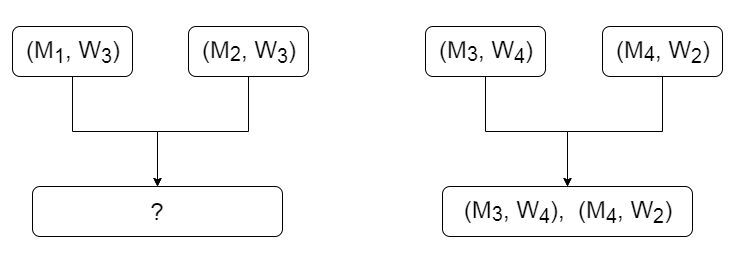
\includegraphics{figures/DivideAndConquer_1.png}}
    \caption{First Merge - Conflict}
    \label{fig:DivideAndConquer_1}
\end{figure}

\begin{figure}[!ht]
    \centering
    \scalebox{.3}{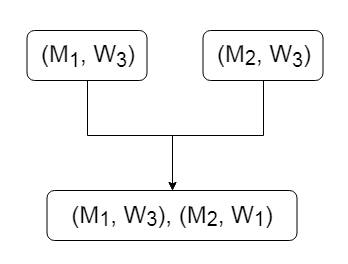
\includegraphics{figures/DivideAndConquer_3.png}}
    \caption{First Merge- Conflict Resolved}
    \label{fig:DivideAndConquer_1}
\end{figure}

\begin{figure}[!ht]
    \centering
    \scalebox{.3}{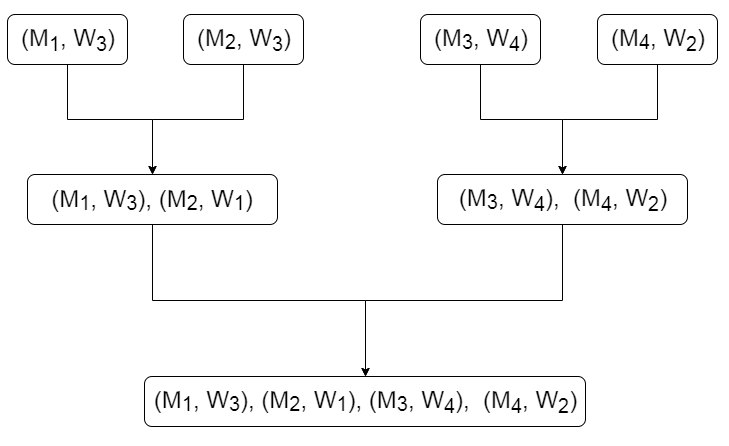
\includegraphics{figures/DivideAndConquer_2.png}}
    \caption{Final Matching}
    \label{fig:DivideAndConquer_1}
\end{figure}




\subsection{Master-Slave Implementation}
The Master-Slave approach to the Gale-Shapely algorithm was based on a model where a master controls all communication between men and women.\cite{larsen1997parallel} The basic algorithm can be thought of in two parts:
\begin{enumerate}
    \item Proposal phase - the master presents all the open proposals to all those receiving proposal requests.
    \item Response phase - in parallel, the ones accepting requests decide the preferred one and return the rejected requests to the master
\end{enumerate}
This process repeats until all matches have been assigned. When evaluating proposals, the master groups proposals together. The slaves are therefor not responding to proposals to one at a time, but as a group. For instance, if a, b, and c all desire x. The master will send all three proposals and x will decide between the three of them right then and there. This is done in a series of rounds so all of the proposer's first preference gets gathered up by the master and sent out. After matches are assigned, all of the proposers who are unassigned have their second preference gathered up and sent out. If a proposer is assigned a match and then rejected, they pick up right where they left off in their proposal position regardless of where their fellow proposers are.


\subsection{Parallel Iterative Improvement Stable Matching Algorithm} Enyue et. al\cite{PII} present a solution for the stable matching problem that deviates considerably from the approach introduced with Gale-Shapley introduced. The approach they published is called Parallel Iterative Improvement (PII) algorithm, and revolves around a ranking matrix built with the preferences of both men and women. The algorithm claims to execute at its best when run on $n^2$ processors.
\subsubsection{Creation of Ranking Matrix}
Figure \ref{fig:PII Ranking Matrix} shows how the initial setting for the PII algorithm is composed. Taking into account a set of preferences for both men and women, a matrix is formed with each field containing a pair build by mixing the preference of a man and a woman. In order to keep a geometrical co-relation between coordinates and matching participants. rows are assigned to men and columns represent women preferences. Men preferences are placed as the left value for each field, whereas women preferences are placed on the right of each field, with the arrangement of preference values being transposed, as each column represents the preference list of a woman.

\begin{figure}[!ht]
    \centering

    \begin{tabular}{lllllllllllllll}
   & \multicolumn{4}{l}{Men's ranking} &  \multicolumn{4}{l}{Women's Ranking}\\
$M_1$ & 4    & 2    & 3    & 1    & $W_1$ & 1     & 4     & 2   & 3 \\
$M_2$ & 3    & 2    & 1    & 4    & $W_2$ & 1     & 2     & 3   & 4  \\
$M_3$ & 2    & 4    & 1    & 3   & $W_3$ & 4     & 2     & 3     & 1  \\
$M_4$ & 1    & 4    & 3    & 2    & $W_4$ & 3     & 1     & 4     & 2 \\
\\

& & &&\multicolumn{3}{l}{Ranking Matrix}\\
 & & & 4,1 & 2,1 & 3,4 & 1,3\\
 &&& 3,4 & 1,2 & 2,2 & 4,1\\
 &&& 2,2 & 4,3 & 1,3 & 3,4\\
 &&& 1,3 & 4,4 & 3,1 & 2,2\\
\end{tabular}\\

    \caption{PII Preference Matrix $n=4$}
    \label{fig:PII Ranking Matrix}
\end{figure}

\subsubsection{Initial Matching}
Initial matching values are assigned randomly. A matching set with the presented matrix configuration has the form of a set of pairs, called \textit{matching pairs}, representing the engagement between the man linked to the row coordinate and the woman linked to the column coordinate. As each matching member can only be matched once, there can only be one matching pair per row and column. The random assignment of initial matching pairs is done via the Random Permutation Algorithm. \cite{Durstenfeld}.
\subsubsection{Iteration Phase}
The most complex part of the algorithm. It consists on the identification of unstable pairs, which are what are normally regarded as blocking pairs. the process of identification requires each pair in the matrix to be compared against the matches on their same row and column, if both preferences in a given pair are higher than the one for the man(left element in the matching pair on the same row) and woman (right element of the matching pair in the same column).\\
Once unstable pairs are identified, two different sets of pairs $NM_1$ and $NM_2$ are computed as described in \cite{PII}. The union of these two values represent the elements to be used in a new matching set, which is completed by adding the initial matching without any pairs in the rows and columns that the new matching pairs are located on.\\
After a new matching set is calculated, all the steps described for the iteration phase are repeated until there are no unstable pairs found. When the different steps in the iteration phase are paralleled, there is a possibility for loops to be generated, where the new matching calculated will have a repeating pattern. One measure to be take in order for this misbehavior to be mitigated is limiting number of times the iterations phase may be executed, and recalculating a Random Permutation initial matching again, starting a new iteration phase with it.

\section{Implementation}
We have made available the source code of all implementations at the repository \url{https://github.com/azeid/StableMatchingParallel}. We provide a description of each implementation and some of the rationale of their design in the following subsections.

\subsection{Parallelization of Gale-Shapley}

As discussed in the introduction section we decided to not modify heavily the basic structure of Gale-Shapley algorithm and instead use some of the concurrent data structure and synchronization mechanism provided by Java. There were three major modifications for the algorithm to be parallelize it.

\begin{enumerate}
    \item The algorithm was encapsulated in a class implementing \texttt{Runnable}. Shared data among workers are 2 integer array to keep track of proposals and engagements, and the two data structures described below.
    \item Instead of a simple \texttt{LinkedList} or \texttt{ArrayList} for keeping track of which men are free. We decided to use a ConcurrentLinkedQueue. This is because the underlying implementation is based on the wait-free algorithm described by Michael and Scott\cite{michael1995simple}. Since the implementation is either removing one element or adding an element and not iterating over it, this was a safe choice.
    \item Last data structure shared among all workers is an array of objects that we use as an array of monitors. 
\end{enumerate}

Given these modifications we were able to run the algorithm in multiple threads using a cached thread pool, and submitting as many workers to the thread pool as there are men in the problem. At this point the reader might be wondering how were the ConcurrentLinkedQueue and the array simple \texttt{Object} used to coordinate all threads.
Let's consider the case of a thread that arrives to the while condition, this list is sort of a ticket and retrieves a number that identifies the work that a man will do. This number will be unique since the list is initialized with all the men in the problem and it is thread-safe. Furthermore is wait-free. Execution of the algorithm continues and for that particular man it will get the identifier of the next woman to propose to. This identifier is used in the array of objects and using the \texttt{synchronized} keyword grabs the intrinsic lock for that object. At this point the rest of the algorithm is guaranteed to be thread safe because any thread only has a unique pair of identifiers for a man and a woman. Therefore is possible for multiple threads to run in parallel as long as they are not trying to propose to the same women. Finally, once the thread finish the proposal-rejection phase goes back to the beginning of the loop and tries to get another man to pair, if the list of free men is empty it simply terminates.

\subsection{Stable Marriage by Coroutines}

For this algorithm we tried different approaches and none of them were successful. This was because our evaluation methodology requires us to use Java for a fair comparison and Java does not natively support coroutines. Although some efforts to modify the Java Virtual Machine and provide an API to support coroutines are available\cite{jkuserializable}\cite{coroutinesoffbynull}, we were unsuccessful in replicating the same behavior of transferring execution control implicitly and preemptively as stated in Allison's algorithm. Another approach we tried was to use a framework of coroutines\footnote{https://github.com/esoco/coroutines} implemented in Java on top of the \texttt{CompletableFuture} class. 
Therefore we excluded this implementation from our evaluations.

\subsection{Divide and Conquer}

\begin{enumerate}
    \item We created a class to encapsulate the internal data structures and merging algorithm. The class implemented the Callable interface. Spawned threads would return 'Future Results' that included the final matching between two matching subsets. 
    \item The top level class encapsulates the following:
    \begin{enumerate}
    \item Two integer arrays for men and women preference lists
    \item An array of type $MatchingPairIndeces$ to hold matchings
    \item A class $MergeTwoMatchingSets$ which has three $MatchingPairIndices$ arrays 'Left', 'Right', and 'Final Matching'. This class takes in two sets and merges them together. Additionally, it has a function to resolve any conflicts.
    \end{enumerate}
\end{enumerate}

\subsubsection{Resolving Conflicts}

Below is the pseudo code for the function that handles resolving matching conflicts.
\begin{figure}[!htb]
    
    \begin{algorithmic}
    \FOR{matching $m$ in currentMatching}
        \IF{currentMatching contains $w$}
            \WHILE{currentMatching contains $w$}
                \IF{$w$ prefers $m$ to her fianc\'e $m\prime$} 
                    \STATE swap $m$ and $m\prime$ matching
                    \STATE match $m\prime$ to his next preference after $w$
                \ELSE
                    \STATE match $m$ to his next preference
                    \STATE add $m$ and $w\prime$ matching to currentMatching
                \ENDIF
            \ENDWHILE
        \ELSE
            \STATE add $m$ and $w$ to currentMatching
        \ENDIF
    \ENDFOR
    \end{algorithmic}
\end{figure}

\subsubsection{Handling Odd Number of Subsets }
If the number of subsets is odd, then the last subset gets cached and added to the final results to make it into the next iteration. The algorithm will eventually gets to 1 final matching set. 

\subsection{PII}
Implementation of this algorithm proved to be more elaborated than initially envisioned. the purpose behind this implementation was to determine whether any improvements could be detected even when not meeting the resources requirement of $n^2$ processors. After the implementation of a sequential variant of this algorithm was completed, it was identified that many areas in the code that would remain sequential after paralleling phases would considerable overhead for the execution time results. Since the equipment considered for the results benchmarking had far less resources than the amount required by the algorithm, It was speculated that the improvements seen by paralleling sections of the code with a small amount of processors would not compensate the overhead of sequential routines, deeming it worthless to complete a parallel implementation of this algorithm considering the amount of effort required to complete the tasks.

\subsection{Master-Slave}
For this implementation we started with a Master-Slave Java pattern using a shared resource. The master (called the matchmaker) queried the proposers for their preference. Then it would group requests so that if a, b, and c all requested x, these requests would be together and sent to a slave to determine the preference of x. This would be for all the proposals. The matchmaker would not progress until all of the proposals that had been sent out had been responded to in one way or another. In the next round, the master would only get the preferences of those proposers who are unmatched and spin up the appropriate threads. Any proposer that had a partner but became unmatched would pick up in the proposal queue where they left off. So even if it was round 4 and the proposer had been matched with their first choice initially, being unmatched would cause the proposer to propose to their second choice. While this implementation passed initial smoke tests of correctness, the full benchmark proved to test the code too much and the bugs could not be resolved. As such, this implementation is mostly complete but buggy and has been excluded from our results.

\section{Evaluation}

\subsection{Methodology}

All of our implementations were written in Java. Initially we thought of measuring the performance of our implementations with a naive approach where we would measure the time either in milliseconds or nanoseconds of solving the stable marriage problem. We could for example simply use \texttt{System.currentTimeMillis()} or \texttt{System.nanoTime()}. However we quickly found out how unreliable the results would be, since we noticed really inconsistent results between runs. As Ponge\cite{architectBenchmarking} explains, this kind of benchmarking might be viable in programs written in statically compiled languages like C. However Java runs on a Virtual Machine and it uses \emph{Just-in-time} compilation, so the first time the code is run it is actually being interpreted and then is compiled to native code, depending on the actual platform that is running. Furthermore, the VM tries to use all kinds of different optimization like loop unrolling, inlining functions or on-stack replacements, making it difficult to get consistent results. \\
We decided to use Java Microbenchmark Harness (JMH)\footnote{http://openjdk.java.net/projects/code-tools/jmh/} for measuring the performance of our implementations. JMH is an open source benchmarking tool part of the OpenJDK. Although it does not entirely prevent all common pitfalls and inconsistencies introduced by the JVM, it does help mitigating them. \\
Next step was to generate some test inputs for our benchmarks. We considered three different scenarios. Best case, where every man $m_i$ and every woman $w_i$ are each other first option. Random case, where the list of preferences for both genders are randomly shuffled. For the worst case we considered McVitie-Wilson\cite{mcvitie1971stable} worst case, Figure \ref{fig:worst_case} shows an example of the rankings for 5 men and women.

\begin{figure}
    \centering
    
    \begin{tabular}{lllllllllllll}
$M_1$ & 1     & 4    & 3    & 2    & 5    &  & $W_1$ & 4     & 3     & 2     & 1    & 5    \\
$M_2$ & 2     & 1    & 4    & 3    & 5    &  & $W_2$ & 1     & 5     & 4     & 3    & 2    \\
$M_3$ & 3     & 2    & 1    & 4    & 5    &  & $W_3$ & 2     & 1     & 5     & 4    & 3    \\
$M_4$ & 4     & 3    & 2    & 1    & 5    &  & $W_4$ & 3     & 2     & 1     & 5    & 4    \\
$M_5$ & 1     & 4    & 3    & 2    & 5    &  & $W_5$ & 5     & 4     & 3     & 2    & 1    \\
   & \multicolumn{5}{l}{Men's ranking} &  &    & \multicolumn{5}{l}{Women's Ranking}
\end{tabular}
    
    \caption{Worst case of stable marriage problem using McVitie-Wilson algorithm when $n=5$}
    \label{fig:worst_case}
\end{figure}

For each case we generated preferences matrices of size $n = {10, 100, 200, 1000}$. There are different modes to run benchmarks in JMH. We decided to measure the average time of an operation in milliseconds, where an operation is solving the stable marriage problem. In this mode, JMH considers an iteration to be a slice of time running as many operations as possible, it measures the time for each operation and averages it. In order to avoid some of the JIT inconsistencies and other JVM  optimizations, JMH runs a few warm-up iterations. After that it runs, by default, 5 iterations where the results are actually recorded. For our measuring purposes we decided to run 3  five seconds warm-up iterations and 5 ten seconds actual iterations.

\subsection{Results}

We ran the benchmark suite in machine with an AMD Ryzen 1700 8-core 16-threads @ 3.6Ghz and 16Gb of DDR4 RAM @ 3,200Mhz. As a baseline we decided to run all the tests in our serial implementation of Gale-Shapley. Results are shows in Table \ref{tab:serial-gale-shapley}. In every cell the amount of milliseconds to complete an operation of the algorithm, i.e. get a result, and the margin of error is specified and a confidence interval of 99\%. 

\begin{table}[h]
    \centering
\begin{tabular}{|l|l|l|l|}
\hline
\multicolumn{1}{|c|}{\textbf{n}} & \multicolumn{1}{c|}{\textbf{Best (ms/op)}} & \multicolumn{1}{c|}{\textbf{Random (ms/op)}} & \multicolumn{1}{c|}{\textbf{Worst (ms/op)}} \\ \hline
10                               & 0.011 ±,0.001                              & 0.014 ±,0.001                                & 0.022 ±,0.001                               \\ \hline
100                              & 0.867 ±,0.009                              & 1.198 ±,0.003                                & 6.595 ±,0.227                               \\ \hline
200                              & 3.463 ±,0.064                              & 5.423 ±,0.238                                & 43.587 ±,0.563                              \\ \hline
1000                             & 87.740 ±,0.628                             & 139.563 ±,3.146                              & 8782.987 ± 3636.943                         \\ \hline
\end{tabular}
    \caption{Serial Gale-Shapley}
    \label{tab:serial-gale-shapley}
\end{table}

We then followed by running our parallel version of Gale-Shapley. Results are shown in Table \ref{tab:parallel-gale-shapley}.


\begin{table}[h]
    \centering
\begin{tabular}{|l|l|l|l|}
\hline
\multicolumn{1}{|c|}{\textbf{n}} & \multicolumn{1}{c|}{\textbf{Best (ms/op)}} & \multicolumn{1}{c|}{\textbf{Random (ms/op)}} & \multicolumn{1}{c|}{\textbf{Worst (ms/op)}} \\ \hline
10                               & 0.176 ±,0.011                              & 0.177 ±,0.004                                & 0.176 ±,0.010                               \\ \hline
100                              & 0.379 ±,0.013                              & 0.376 ±,0.011                                & 1.082 ±,0.009                               \\ \hline
200                              & 0.564 ±,0.022                              & 0.728 ±,0.059                                & 5.576 ±,0.106                               \\ \hline
1000                             & 2.115 ±,0.023                              & 3.751 ±,0.168                                & 482.950 ±,31.277                            \\ \hline
\end{tabular}
    \caption{Parallel Gale-Shapley}
    \label{tab:parallel-gale-shapley}
\end{table}

Finally we ran our approach to divide and conquer in parallel. Results are shown in Table \ref{tab:parallel-tseng-lee}

\begin{table}[h]
    \centering
\begin{tabular}{|l|l|l|l|}
\hline
\multicolumn{1}{|c|}{\textbf{n}} & \multicolumn{1}{c|}{\textbf{Best (ms/op)}} & \multicolumn{1}{c|}{\textbf{Random (ms/op)}} & \multicolumn{1}{c|}{\textbf{Worst (ms/op)}} \\ \hline
10                               & 0.168 ±,0.003                              & 0.169 ±,0.007                                & 0.174 ±,0.013                               \\ \hline
100                              & 0.691 ±,0.007                              & 1.008 ±,0.035                                & 1.999 ±,0.025                               \\ \hline
200                              & 2.153 ±,0.034                              & 3.773 ±,0.150                                & 8.559 ±,0.304                               \\ \hline
1000                             & 43.971 ±,0.752                             & 74.536 ±,2.207                               & 401.745 ±,7.819                             \\ \hline
\end{tabular}
    \caption{Parallel Tseng-Lee}
    \label{tab:parallel-tseng-lee}
\end{table}

There a few things important to notice in these results. First, observe how the serial version is much faster than both parallel implementations for a small $n$, such as $n=10$. This is due to the overhead introduced of running multiple threads. One can observe also that the payoff of a parallel approach starts to have a significant payoff when $n \geq 100$. Another outstanding result is how fast is our implementation of parallel Gale-Shapley compared to parallel divide and conquer and of course the serial version, for the best and random case. However for the worst case both parallel algorithms seem to have a similar performance.

\section{Future Work}
In the effort of having more algorithms to evaluate and compare against the results reported in this paper, implementation of the Parallel Iterative Improvement algorithm can be revisited. Additionally, we believe that using a profiler to check for possible optimizations would also improve our results. The proposed course of action would be to implement this algorithm with CUDA, to make use of a GPUs numerous cores, in an effort to be as close as possible to the $n^2$ processors listed as the ideal resources for the algorithm. Current GPUs would enable realistic results to be obtained for $n$ ranging  up to multiple tens.
To go alone with that effort, finishing debugging and optimizing of the Master-Slave algorithm would be on the list as well (in addition to being the most attainable). This implementation could do with refining and debugging in order to run it against the other implementations. However, because of the bottleneck of the master I expect it to perform worse overall especially in the worst case-scenario.
Having more robust ways to measure effectiveness would help as well. While our benchmarking framework is effective and informative, there are always other things that can be looked. In addition, our implementations may be optimized and allow us to obtain even cleaner results.

\section{Conclusion}
As you can see from the table, Serial Gale-Shapley is the unquestioned champion in a situation where there very few n. It outstripped the others easily, but quickly falls off as more participants get added. As the non-parallel algorithm is already fairly fast for low n this is an underwhelming result, however we could see it being a very effective method for calculating the matching of a large number of small groups. Parallel Gale-Shapley performs better in almost all situations than the other two making it the most well-rounded of the algorithms. It is worth mentioning, that Tseng-Lee outperforms Gale-Shapley in the worst-case scenario with n equal to 1000 albeit only slightly.

\bibliographystyle{plain}
\bibliography{references}

\end{document}
